Este problema, obtenido en la página web tutorial de Qiskit~\cite{qiskit_tutorial_antiguo}, consiste en resolver max-cut para el grafo de la \textit{fig.~\ref{fig:4-qiskit grafo}}, que consiste en, asignando un valor 0 o 1 a cada nodo maximizar la cantidad de aristas entre nodos de distinto valor.

\begin{figure}[Grafo {--} max-cut en grafo de 4 aristas]{fig:4-qiskit grafo}{Grafo del problema\cite{qiskit_tutorial_antiguo}}
  \centering
  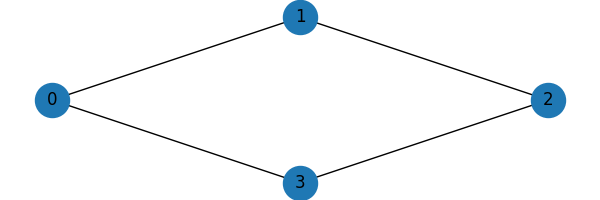
\includegraphics[scale=0.75]{qiskit-grafo/qiskit-grafo.png}
\end{figure}

Se parte de este caso por tratarse de uno sencillo.
Esto es porque la cantidad de qubits es pequeña y no existen restricciones en este problema, por lo que el espacio de estados válidos disponibles es de $2^4$.
Estas condiciones hacen que el algoritmo trabaje sobre un circuito pequeño, tanto en profundidad como en número de qubits, lo que reduce el ruido y facilita su implementación. 

\begin{itemize}
\item \textbf{Formulación:} \\
  Sea $G = (V, E)$ el grafo de la \textit{fig.~\ref{fig:4-qiskit grafo}}, con $V = [0, 1, 2, 3]$ y $E = [(0, 1), (1, 2), (2, 3), (0, 3)]$ los nodos y aristas de G respectivamente.

  Sea $x_i \in \{0, 1\}$ el color del nodo $i$.

\item \textbf{Objetivo:} \\
  \begin{align}\label{eq:4-tutorial qiskit objetivo}
    \max(\sum_{(i, j) \in E} (x_i * (1 - x_j) + x_j * (1 - x_i)))
  \end{align}

\end{itemize}

Como \textit{QAOA} sirve para encontrar el mínimo de una función, se multiplicará la (\textit{ecuación \ref{eq:4-tutorial qiskit objetivo}}) $*-1$.
\\
De esta forma se tiene que la función de coste a minimizar para este problema en particular es la siguiente:

\begin{align}
  f(x) = \sum_{(i, j) \in E} (x_i * (x_j - 1) + x_j * (x_i - 1))
\end{align}

Así, cada cláusula del sumatorio será $-1$ para una arista con dos nodos de distinto valor y 0 en otro caso.

Como el problema no tiene restricciones y las variables de entrada son $x_i \in \{0, 1\}$, el problema ya se encuentra en formato QUBO\@.
El paso a formato Ising se realiza de acuerdo con lo descrito en la \textit{sección~\ref{sec:3-operador_c}}.
Utilizando el cambio de variable $x_i \rightarrow \frac{1 - z_i}{2}$ se genera la siguiente función $g(z)$:

\begin{align}
  g(z) &= \sum_{(i, j) \in E} (\frac{1 - z_i}{2} * (\frac{1 - z_j}{2} - 1) + \frac{1 - z_j}{2} * (\frac{1 - z_i}{2} - 1)) = \sum_{(i, j) \in E} \frac{z_i z_j - 1}{2}
\end{align}

Como ha sido explicado en la \textit{sección~\ref{sec:3-operador_c}} y demostrado en la \textit{sección~\ref{CAP:F_CLASICA_A_HAMILTONIANO}} del apéndice, para obtener el operador $C$ se deben sustituir las variables $z_i$ por puertas $\sigma^z_i$.
Además se debe tener en cuenta que debido al postulado de medición en mecánica cuántica\cite{Nielsen_Chuang_2010} la fase global es despreciable.
\\
Esto significa que dado un operador lineal $A$ y $n \in \mathbb{R}$: $e^{i \gamma n} \cdot e^{i \gamma A} = e^{i \gamma A}$

Y teniendo en cuenta las siguientes definiciones:
\begin{itemize}
\item $ Rz_i(\lambda) = \exp(-i\frac{\lambda}{2}\sigma_i^z) $
\item $ Rz_i z_j(\lambda) = \exp(-i\frac{\lambda}{2}\sigma_i^z \otimes \sigma_j^z) $
\end{itemize}

Se obtiene:

\begin{align}
  U(C, \gamma) &=  \exp(-i*\gamma*C) = \exp(-i*\gamma* \sum_{(i, j) \in E} \frac{\sigma_i^z \otimes \sigma_j^z - 1}{2}) = \nonumber \\
          &= \prod_{(i, j) \in E} \exp(-i*\gamma* \frac{\sigma_i^z \otimes \sigma_j^z - 1}{2}) = \nonumber \\
          &= \prod_{(i, j) \in E} [ \exp(-i*\frac{\gamma}{2}* \sigma_i^z \otimes \sigma_j^z) * \exp(i*\frac{\gamma}{2}) ] = \nonumber \\
          &= \prod_{(i, j) \in E} Rz_i z_j(\gamma)
\end{align}

Con el operador \(U(B, \beta)\) y el vector inicial, definidos en la \textit{sección~\ref{sec:3-circuito de qaoa}}, y el operador \(U(C, \gamma)\) obtenido se puede construir el circuito cuántico.

\paragraph{Discusión de la diferencia entre circuitos de distintas implementaciones de QAOA}

\begin{figure}[Circuito {--} max-cut en grafo de 4 aristas propio]{fig:4-qiskit_circuito}{ Circuito obtenido con la implementación de QAOA del TFG ($p=1$) }
  \centering
  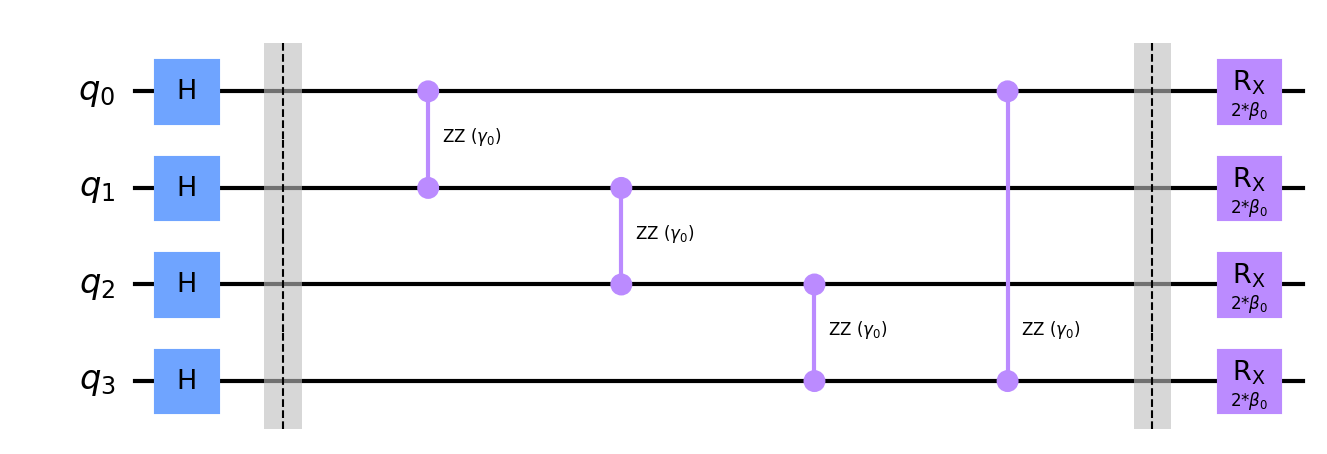
\includegraphics[scale=0.6]{circuits/qiskit/qiskit-circuit-2gamma-p1.png}
\end{figure}

\begin{figure}[Circuito {--} max-cut en grafo de 4 aristas de la fuente]{fig:4-qiskit_tutorial_circuito}{ Circuito de ejemplo de la página web\cite{qiskit_tutorial_antiguo} ($p=1$) }
  \centering
  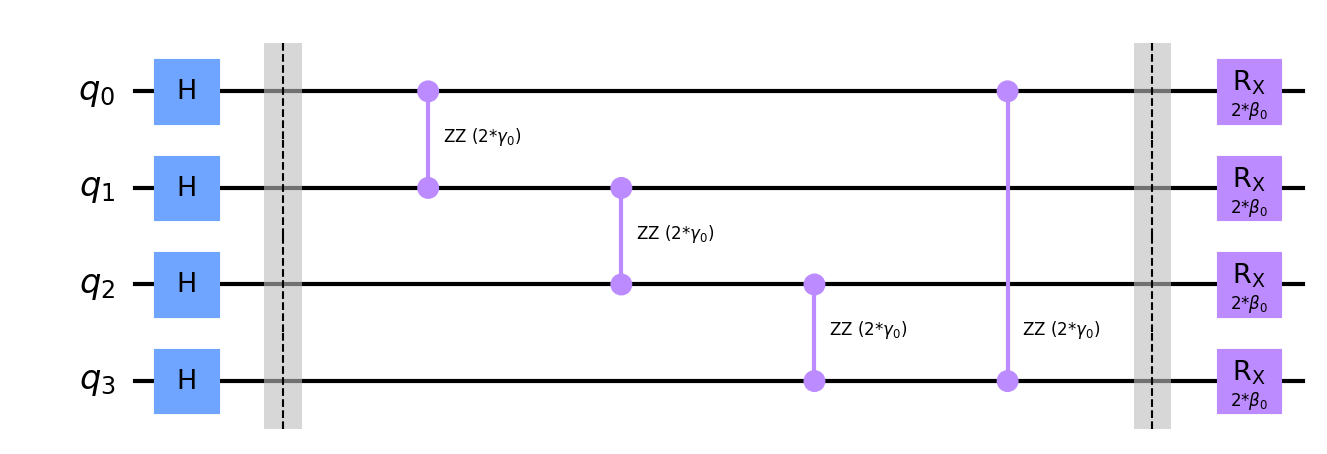
\includegraphics[scale=0.6]{circuits/qiskit/tutorial-qiskit-circuit-2gamma-p1.png}
\end{figure}

\begin{figure}[Circuito {--} max-cut en grafo de 4 aristas de QAOAAnsatz]{fig:4-qiskit_QAOAAnsatz_circuito}{ Circuito generado por QAOAAnsatz ($p=1$) }
  \centering
  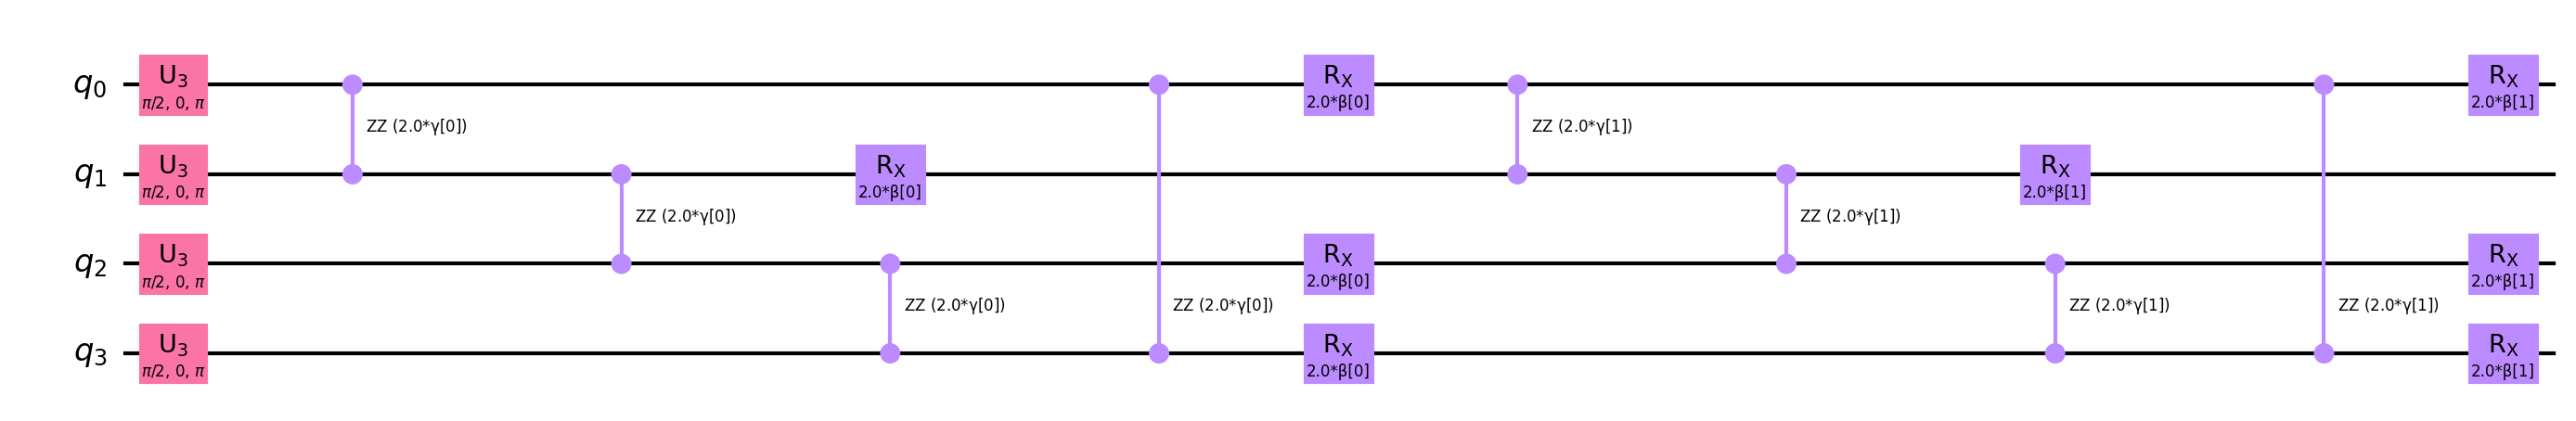
\includegraphics[scale=0.6]{circuits/qiskit/qiskit-circuit-qaoaAnsatz-p1.png}
\end{figure}

El circuito generado con el desarrollo de este TFG (\textit{fig.~\ref{fig:4-qiskit_circuito}}) y el generado por la función \textit{QAOAAnsatz} de la librería Qiskit (\textit{fig.~\ref{fig:4-qiskit_QAOAAnsatz_circuito}}) son equivalentes.
Las diferencias son únicamente visuales con respecto a la disposición de las puertas.

El circuito obtenido de la página web tutorial de Qiskit\cite{qiskit_tutorial_antiguo} (\textit{fig.~\ref{fig:4-qiskit_tutorial_circuito}}) corresponde a desarrollar los mismos cálculos solo que con $f_2(x) = 2*f(x)$ como función de coste.
\\
Aunque las puertas \textit{Rzz} tengan coeficientes distintos ambas son correctas.
Esto es porque ambos circuitos resultantes tienen un mismo estado fundamental, solo que uno lo tiene con el doble de energía que el otro.
En otras palabras ambas funciones $f_2$ y $f$ tienen un mismo $x$ que las minimiza.


%%% Local Variables:
%%% mode: latex
%%% TeX-master: "../tfgtfmthesisuam"
%%% End:
